\documentclass[11pt]{charter}

% El títulos de la memoria, se usa en la carátula y se puede usar el cualquier lugar del documento con el comando \ttitle
\titulo{Estimación de la captura realizada en buques pesqueros mediante visión artificial} 

% Nombre del posgrado, se usa en la carátula y se puede usar el cualquier lugar del documento con el comando \degreename
%\posgrado{Carrera de Especialización en Sistemas Embebidos} 
%\posgrado{Carrera de Especialización en Inteligencia  de las Cosas} 
\posgrado{Carrera de Especialización en Inteligencia Artificial}
%\posgrado{Maestría en Sistemas Embebidos} 
%\posgrado{Maestría en Internet de las cosas}

% Tu nombre, se puede usar el cualquier lugar del documento con el comando \authorname
\autor{Lic. Nicolás Eduardo Horro} 

% El nombre del director y co-director, se puede usar el cualquier lugar del documento con el comando \supname y \cosupname y \pertesupname y \pertecosupname
\director{Dr. Félix Ramón Rojo}
\pertenenciaDirector{INVAP S.E.} 
% FIXME:NO IMPLEMENTADO EL CODIRECTOR ni su pertenencia
%\codirector{} % si queda vacio no se deberíá incluir 
%\pertenenciaCoDirector{}

% Nombre del cliente, quien va a aprobar los resultados del proyecto, se puede usar con el comando \clientename y \empclientename
\cliente{Dr. Jorge Omar Lugo}
\empresaCliente{INVAP S.E.}

% Nombre y pertenencia de los jurados, se pueden usar el cualquier lugar del documento con el comando \jurunoname, \jurdosname y \jurtresname y \perteunoname, \pertedosname y \pertetresname.
\juradoUno{Nombre y Apellido (1)}
\pertenenciaJurUno{pertenencia (1)} 
\juradoDos{Nombre y Apellido (2)}
\pertenenciaJurDos{pertenencia (2)}
\juradoTres{Nombre y Apellido (3)}
\pertenenciaJurTres{pertenencia (3)}
 
\fechaINICIO{05 de agosto de 2021}		%Fecha de inicio de la cursada de GdP \fechaInicioName
\fechaFINALPlanificacion{13 de marzo de 2021} 	%Fecha de final de cursada de GdP
\fechaFINALTrabajo{23 de abril de 2021}		%Fecha de defensa pública del trabajo final


\begin{document}

\maketitle
\thispagestyle{empty}
\pagebreak


\thispagestyle{empty}
{\setlength{\parskip}{0pt}
\tableofcontents{}
}
\pagebreak


\section{Registros de cambios}
\label{sec:registro}


\begin{table}[ht]
\label{tab:registro}
\centering
\begin{tabularx}{\linewidth}{@{}|c|X|c|@{}}
\hline
\rowcolor[HTML]{C0C0C0} 
Revisión & \multicolumn{1}{c|}{\cellcolor[HTML]{C0C0C0}Detalles de los cambios realizados} & Fecha      \\ \hline
1.0      & Creación del documento                                          & 05/03/2021 \\ \hline
1.1      & Avances en alguna cosa                                          & dd/mm/aaaa \\ \hline
1.2      & Otro ejemplo \newline
		   Con texto partido \newline
		   En varias líneas \newline
		   A propósito                                                     & dd/mm/aaaa \\ \hline
\end{tabularx}
\end{table}

\pagebreak

\section{Acta de constitución del proyecto}
\label{sec:acta}

\begin{flushright}
San Carlos de Bariloche, \fechaInicioName
\end{flushright}

\vspace{2cm}

Por medio de la presente se acuerda con el Lic. \authorname\hspace{1px} que su Trabajo Final de la \degreename\hspace{1px} se titulará ``\ttitle'', consistirá esencialmente en el prototipo preliminar de un sistema para clasificación de capturas y descarte en buques pesqueros utilizando técnicas visión por computadora e inteligencia artificial, y tendrá un presupuesto preliminar estimado de 600 hs de trabajo, con fecha de inicio \fechaInicioName\hspace{1px} y fecha de presentación pública \fechaFinalName.

Se adjunta a esta acta la planificación inicial.

\vfill

% Esta parte se construye sola con la información que hayan cargado en el preámbulo del documento y no debe modificarla
\begin{table}[ht]
\centering
\begin{tabular}{ccc}
\begin{tabular}[c]{@{}c@{}}Ariel Lutenberg \\ Director posgrado FIUBA\end{tabular} & \hspace{2cm} & \begin{tabular}[c]{@{}c@{}}\clientename \\ \empclientename \end{tabular} \vspace{2.5cm} \\ 
\multicolumn{3}{c}{\begin{tabular}[c]{@{}c@{}} \supname \\ Director del Trabajo Final\end{tabular}} \vspace{2.5cm} \\
%\begin{tabular}[c]{@{}c@{}}\jurunoname \\ Jurado del Trabajo Final\end{tabular}     &  & \begin{tabular}[c]{@{}c@{}}\jurdosname\\ Jurado del Trabajo Final\end{tabular}  \vspace{2.5cm}  \\
%\multicolumn{3}{c}{\begin{tabular}[c]{@{}c@{}} \jurtresname\\ Jurado del Trabajo Final\end{tabular}} \vspace{.5cm}                                                                     
\end{tabular}
\end{table}

\section{Descripción técnica-conceptual del proyecto a realizar}
\label{sec:descripcion}

El presente proyecto consiste en un prototipo que extiende el Sistema de Monitoreo Electrónico (SME) que incluye sistemas de Circuitos Cerrados de Televisión (CCTV) a bordo de los buques pesqueros mediante el uso Inteligencia Artificial (IA). El objetivo es la automatización del proceso de clasificación y estimación de cantidad de piezas capturadas y descartadas, proceso que actualmente se realiza de manera manual y resulta costoso y propenso a errores. Esta tarea se realiza mediante inspección y es llevada a cabo por operadores humanos.

La figura  \ref{fig:canvas} muestra un diagrama de lienzo (canvas) del modelo de negocio de la solución, que se se explicará con mayor detalle a continuación.

\vspace{25px}

\begin{figure}[htpb]
\centering 
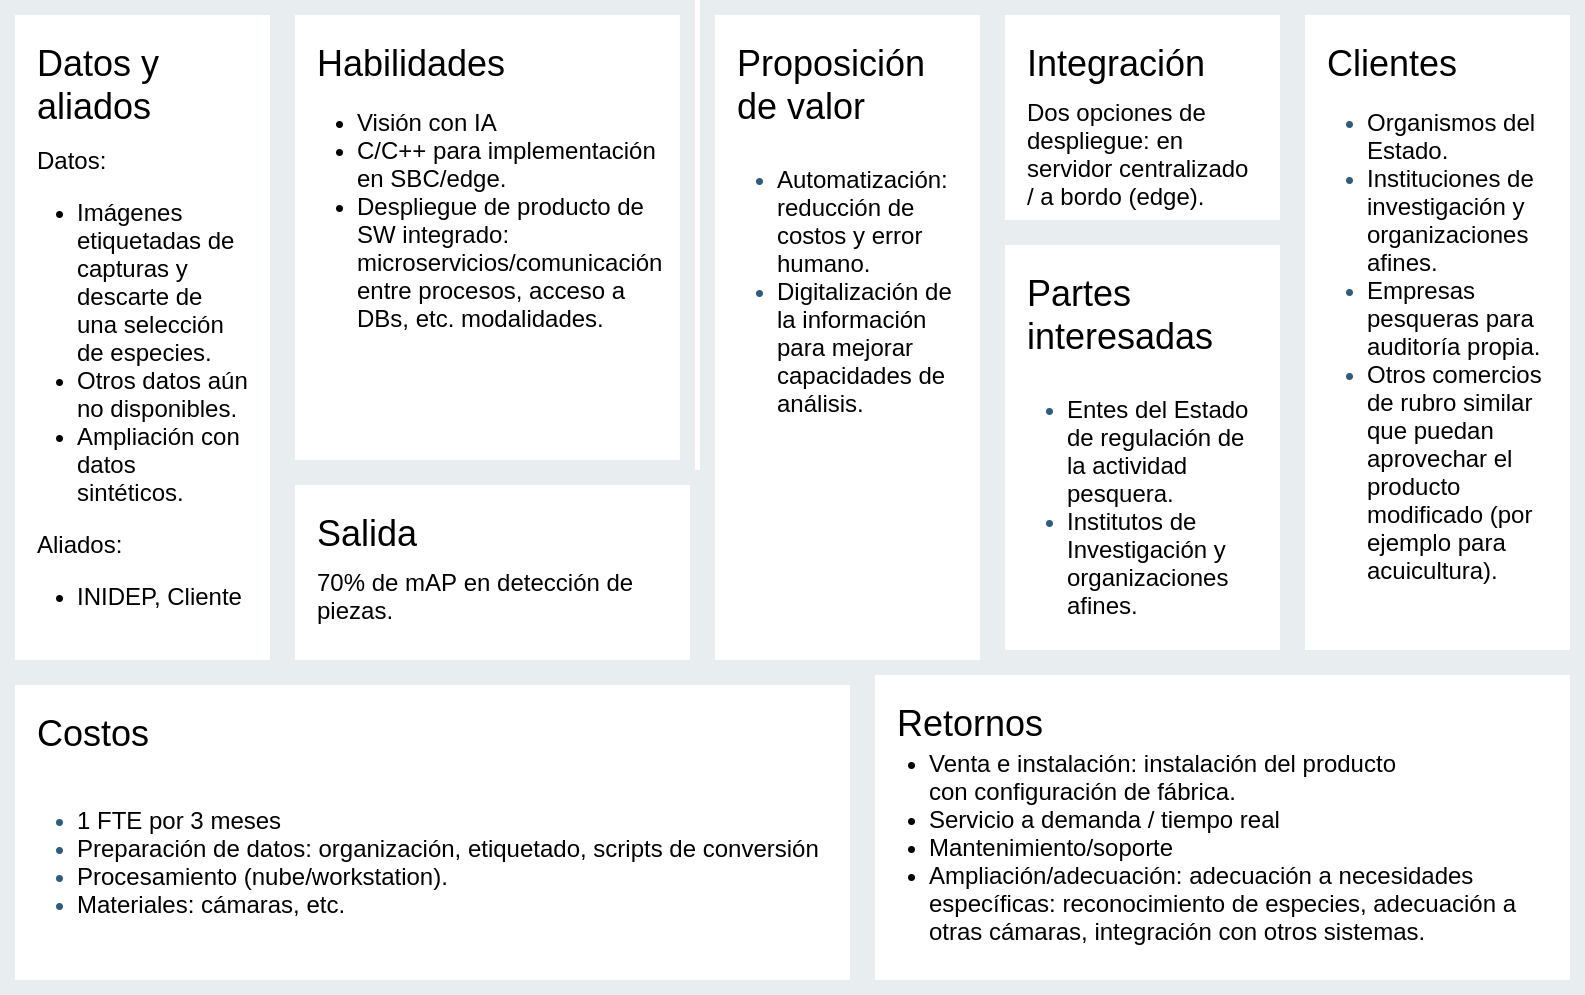
\includegraphics[width=1\textwidth]{./Figuras/canvas.png}
\caption{Diagrama de lienzo (canvas) del modelo de negocio de la solución}
\label{fig:canvas}
\end{figure}

\vspace{25px}

\subsection{Introducción general al tema}

La pesca industrial es un tipo de pesca que tiene como objetivo obtener un gran número de capturas. En Argentina el sector primario pesquero (aquél que se ocupa de la captura) se compone de una flota de buques fresqueros de altura, de costeros grandes y costeros chicos y una flota de buques procesadores. La flota fresquera de altura está conformada por barcos arrastreros con bodegas refrigeradas y cuentan con equipamiento de navegación y detección y utilizan redes de arrastre.

La figura \ref{fig:tipo_embarcaciones} expone un diagrama simplificado de los tipos de embarcaciones y métodos de captura de acuerdo a la profundidad.

\vspace{25px}

\begin{figure}[htpb]
\centering 
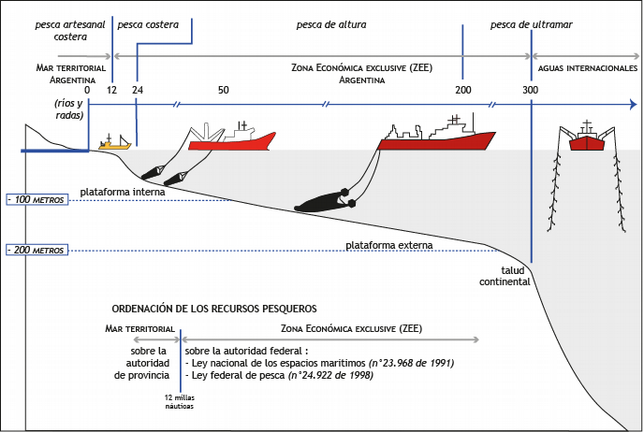
\includegraphics[width=.7\textwidth]{./Figuras/tipo_embarcaciones.png}
\caption{Tipos de embarcaciones según el tipo de pesca}
\label{fig:tipo_embarcaciones}
\end{figure}

\vspace{25px}

A fin de garantizar que la pesca a esta escala sea sostenible, el Consejo Federal Pesquero tiene como funciones el establecimiento de la política pesquera y de la política de investigación pesquera nacional, la planificación del desarrollo pesquero nacional, el establecimiento de la Captura Máxima Permisible (CMP) por especie y las cuotas de captura, así como aprobar los permisos de pesca comercial y experimental y fijar los cánones por el ejercicio de la pesca, entre otros. 
Dado que una pesquería es un sistema complejo de factores interdependientes entre los que se cuentan el estado del recurso biológico, limitaciones sociales e institucionales, condiciones económicas y convicciones culturales, etc., es importante generar información estadística e indicadores que permitan el análisis de la actividad de las pesquerías para poder establecer de manera precisa su marco regulatorio.
El monitoreo y la vigilancia deben permitir conocer las características del esfuerzo en la actividad pesquera y asegurar que las capturan se realicen dentro de los cánones admitidos. Existen también regulaciones que establecen el modo en que debe emplearse la técnica, por ejemplo, exigiendo una permanencia mínima de las redes en el fondo para disminuir la captura incidental de mamíferos marinos.
Tradicionalmente, la principal manera de recopilar información independiente acerca de las actividades y la captura de los buques ha sido mediante observadores a bordo, pero existe una creciente tendencia a la utilización de sistemas electrónicos y un mayor grado de automatización.
El Seguimiento Electrónico (EM) se presenta como una alternativa eficiente y rentable.
Si bien el registro y monitoreo digital de las actividades a bordo representa un avance respecto a la elaboración de reportes manuscritos, el análisis de la cantidad datos generados, la manipulación de sus medios de almacenamiento y la dependencia de observadores calificados para su análisis, no deja de ser una alternativa costosa y también propensa a otro tipo de errores.

Las nuevas técnicas en las áreas de Visión por Computadora e Inteligencia Artificial hallan un posible campo de aplicación en la optimización de estas tareas de análisis, como lo demuestran algunos trabajos con resultados alentadores. Por otra parte, el conocido sitio de competencias de aprendizaje automático Kaggle realizó una competencia de clasificación de capturas en buques pesqueros también con el tema de  combatir la sobreexplotación del recurso.

El presente proyecto se destaca especialmente por incorporar estas técnicas para lograr un mayor grado de automatismo. Esto lo diferencia de otros sistemas similares en los que se requiere de mayor participación de personal calificado.

La figura \ref{fig:seguimiento_electronico} muestra un esquema de un sistema de seguimiento electrónico típico y algunos ejemplos de sus usos.

\vspace{25px}

\begin{figure}[htpb]
\centering 
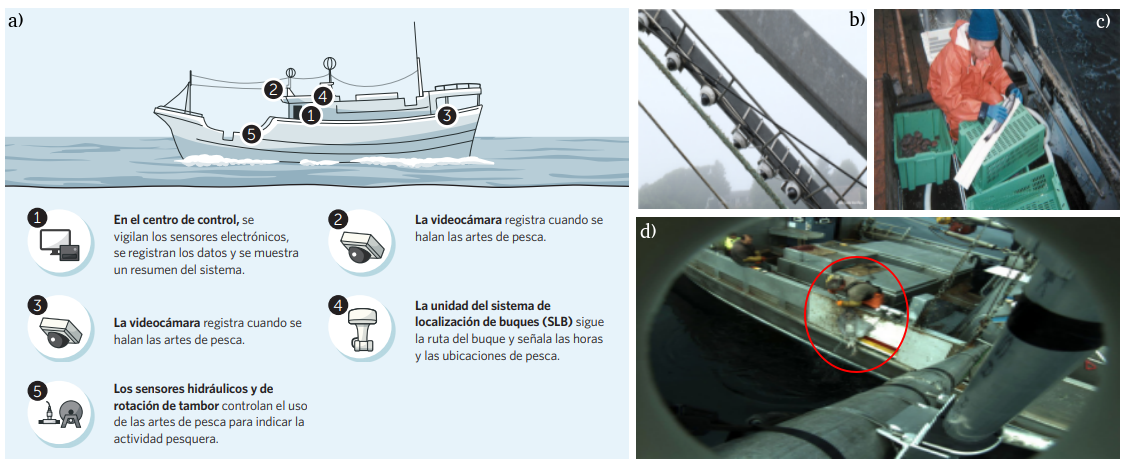
\includegraphics[width=.7\textwidth]{./Figuras/seguimiento_electronico.png}
\caption{ a) Sistema de Seguimiento Electrónico. b) Sistema de CCTV apuntando a redes de arrastre. c) Registro de especímenes por observadores calificados. d) Cámara captando descarte de especie protegida, probablemente no declarada.}
\label{fig:seguimiento_electronico}
\end{figure}

\vspace{25px}

\subsection{Marco de la propuesta}

INVAP S.E. es una empresa del Gobierno de Río Negro dedicada al diseño y construcción de sistemas tecnológicos complejos, con una trayectoria de cuatro décadas en el mercado nacional y tres en la escena internacional. La empresa define como su misión el desarrollo de tecnología de avanzada en diferentes campos de la industria, la ciencia y la investigación aplicada, creando “paquetes tecnológicos” de alto valor agregado tanto para satisfacer necesidades nacionales como para insertarse en mercados externos a través de la exportación.
Dentro del contexto de la búsqueda de nuevos negocios e incorporación de nuevas tecnologías, se realizan trabajos de investigación y prototipos, a menudo mediante convenios con universidades y otras organizaciones, ya sea en calidad de pasantías, prácticas profesionales, trabajos de carreras de grado y posgrado, u otros. Estos trabajos pueden eventualmente evolucionar y aprovecharse en un proyecto de mayor envergadura.
El proyecto que se describe es uno de estos casos y se integra en un desarrollo de mayor alcance: un sistema de monitoreo electrónico que utiliza cámaras de video y computadoras o dispositivos auxiliares para el control de la pesca. Existe un plan de incorporar gradualmente mayores niveles de automatismo y capacidades de reporte en tiempo real a este sistema. 
El principal cliente interesado es el Estado Argentino, y en particular la Subsecretaría de Pesca y Acuicultura perteneciente a la Secretaría de Agricultura, Ganadería y Pesca del Ministerio de Agricultura, Ganadería y Pesca. Si bien no son clientes directos, es también importante mencionar la participación del Consejo Federal Pesquero (https://cfp.gob.ar/) y de INIDEP(https://www.argentina.gob.ar/inidep), organismos involucrados en el seguimiento y regulación de la explotación del recurso y promotores de la modernización de los sistemas de monitoreo y seguimiento. También pueden ser potenciales usuarios centros de investigación o entes privados que lo utilicen para registro propio. El desarrollo y vinculación con instituciones se realiza por medio de INVAP S.E.
Como se mencionó, este trabajo es un subproducto de un proyecto de mayor envergadura. El desarrollo actual de INVAP S.E. tiene como objetivos posibilitar el registro de video y de la información de otros dispositivos (por ejemplo motores de las redes de arrastre) para su posterior análisis en tierra (dependiendo del caso puede ser hasta luego de 30 días en el mar). La segunda etapa del desarrollo es el procesamiento y envío del parte de pesca en tiempo real, y por último la automatización de algunas tareas de análisis. Este trabajo es un prototipo para esta última etapa. 

\subsection{Descripción del proyecto}

La distorsión de lente de pez que suelen tener las cámaras de vigilancia, las condiciones de iluminación variables (zonas de escaso contraste por la fuerte saturación de luces fluorescentes y otras casi sin iluminar) y la dificultad para detectar una estructura por la forma y disposición de las presas hacen que resulte difícil garantizar una correcta detección por un método automático.

La figura \ref{fig:ejemplos_escenas} muestra ejemplos de los tipos de escenas en las cuales se apunta a realizar la detección.

\vspace{25px}

\begin{figure}[htpb]
\centering 
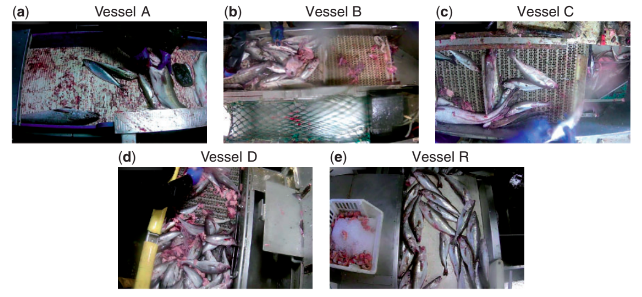
\includegraphics[width=.7\textwidth]{./Figuras/ejemplos_escenas.png}
\caption{Comparación de imágenes de cámaras en distintos buques. La orientación aleatoria de las presas y su mutua oclusión, y la difícil estructura de la escena presentan un desafío para los algoritmos de detección}
\label{fig:ejemplos_escenas}
\end{figure}

\vspace{25px}

Aún así, la literatura consultada muestra que se pueden obtener resultados aceptables utilizando alguna variante de red convolucional (CNN, por sus siglas en inglés Convolutional Neural Network). 
Una característica de las redes neuronales profundas es que requieren una gran cantidad de datos de entrenamiento, que en este caso (a diferencia de como ocurre en otros dominios, como el reconocimiento de personas, caras, vehículos, carteles, etc.) es difícil (o costoso) obtener.

La innovación de esta propuesta reside en la aplicación del estado del arte de estas técnicas a un dominio para el cuál no existen productos o soluciones en el mercado.

La solución propuesta se compone de los siguientes bloques:

\begin{itemize}
\item Ingesta de Video: obtiene la los cuadros de una cámara o un archivo de video y aplica una corrección de imagen para reducir las diferencias entre cámaras. Esta corrección puede incluir: contrarrestar distorsión de lente de pez, aplicar transformaciones de coordenadas cromáticas, ecualizar la imagen, etc.

\item Detección: este bloque recibe los cuadros de video procesados de la etapa anterior y por cada cuadro extrae las regiones de interés y la probabilidad de que exista alguna de las clases detectadas. Se utilizará el algoritmo YOLOv4 o variantes del mismo, dado que representa el estado del arte y es apto para procesamiento en tiempo real si se dispone del HW apropiado. A menudo la capacidad de detección de un objeto puede depender de su orientación, condiciones de oclusión, iluminación, etc. Es posible que un objeto que no sea fácilmente identificable en un cuadro de video, sí lo sea en otros cuadros de ese mismo video. Para este trabajo se propone usar un algoritmo de seguimiento que también representa el estado del arte, denominado DeepSORT. La salida de este algoritmo es una trayectoria de un objeto. Como etapa final, se propone un filtro para decidir si rechazar o no la detección y asociar un evento a esa trayectoria (por ejemplo, incrementar un contador de capturas, reportar un descarte, etc.).

\item Información de contexto (opcional): se puede utilizar información de localización del buque, fecha y hora, actividad de sistemas mecánicos y otros datos tanto para acompañar la salida del clasificador como para mejorarla, dado que hay especies que habitan determinados sectores o se capturan a determinada profundidade intervienen sistemas de captura específicos para un tipo de objetivo.

\item Registro y Generación de Reportes: la salida de la etapa anterior es registrada en una base de datos, para obtener trazabilidad de las capturas y descartes (horarios, tipos de capturas, cantidad de descartes, etc.). Para facilitar el consumo de esta información y permitir combinarla con otros servicios, se utilizará una base de datos con interfaz REST (por ejemplo InfluxDB).
\end{itemize}

La figura  \ref{fig:diagrama_bloques} muestra un diagrama de bloques de la solución propuesta.

\vspace{25px}

\begin{figure}[htpb]
\centering 
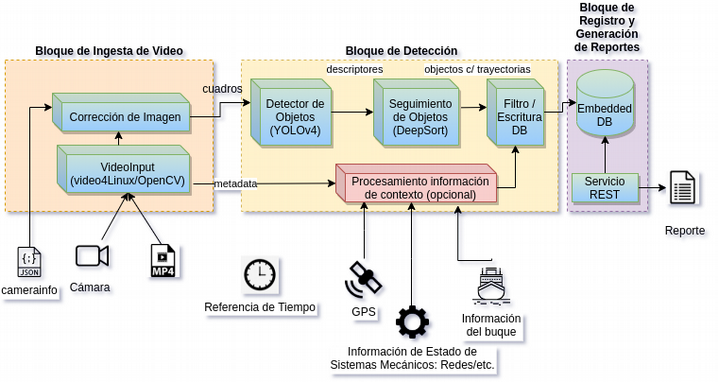
\includegraphics[width=.7\textwidth]{./Figuras/diagrama_bloques.png}
\caption{Diagrama en bloques del sistema}
\label{fig:diagrama_bloques}
\end{figure}

\vspace{25px}

\section{Identificación y análisis de los interesados}
\label{sec:interesados}

\section{1. Propósito del proyecto}
\label{sec:proposito}

En línea con una estrategia de continua mejora e innovación, el propósito de este proyecto es incorporar al proyecto del sistema de seguimiento de pesca que está siendo actualmente desarrollado por INVAP S.E. un componente adicional para la automatización de las tareas de registro e inspección. 

\section{2. Alcance del proyecto}
\label{sec:alcance}

El presente proyecto contempla todo el software a desarrollar para el ciclo completo que se expuso en la figura \ref{fig:diagrama_bloques} desde la adquisición de una imagen (utilizando los drivers o formato de publicación de las cámaras) hasta el reporte almacenado en las bases de datos. Hay una parte del hardware que ya está definida / o fuera del alcance (por ejemplo cámaras y algunas de las computadoras). Es parte de la solución recomendar un ambiente de ejecución.
Dado que el objetivo de este proyecto es estudiar la viabilidad técnica, dependiendo de los datos que puedan obtenerse de buques operativos o datos históricos, se seleccionará un subconjunto de especies a clasificar del total de las reportadas por INIDEP. Dado que cada especie tiene características especiales que permiten distinguirla, se realizará un estudio e ingeniería de características sobre esta selección para tratar de aprovecharlas en el algoritmo clasificador, incluyendo el arte de pesca y zonas de captura para obtenerlas -que determina el tipo de buque-, horario y temporada, parámetros operativos de los sistemas mecánicos de redes de arrastre (en caso que apliquen) y otros. Se utilizará como principal fuente de información la aportada por el cliente y será complementada con reportes e informes de INIDEP. 


\section{3. Supuestos del proyecto}
\label{sec:supuestos}

Para el desarrollo del presente proyecto se supone que:

\begin{itemize}
\item Se contará con los datos necesarios. Se recomienda para contar con un mínimo de 2000 ejemplos por cada clase de objeto a detectar. Si no pudiera alcanzarse este número, existen técnicas para compensar la falta de datos, pero puede verse penalizado el desempeño final del algoritmo y su capacidad de generalizar, siendo necesario un trabajo de ingeniería de features dependiendo de las características de las escenas en los que se utilizará.
\item Contando con datos de cantidad y calidad suficiente, los algoritmos de la familia YOLOv4 y DeepSORT son aptos para resolver esta tarea con un desempeño igual o ligeramente superior al de un operador humano o de un mAP de 70\%.
\item Se contará con el HW disponible para desarrollo y ejecución del proyecto.
\end{itemize}

\section{4. Requerimientos}
\label{sec:requerimientos}

\begin{enumerate}
\item Requerimientos generales
	\begin{enumerate}
	\item El sistema debe complementar una solución existente de hasta 4 cámaras de videos, para automatizar operaciones de conteo que se hacen sobre las mismas por operadores humanos.
	\end{enumerate}
\item Requerimientos funcionales
	\begin{enumerate}
	\item El sistema debe poder ingestar video almacenado y en vivo en formato de color RGB y a resoluciones entre los 360p y 1080p. 
	\item El sistema debe detectar regiones de la imagen conteniendo presas (pescados) en una escena con un porcentaje de confianza. El tipo de presas a detectar depende de como se haya configurado y entrenado el detector en cada caso.
	\item El sistema debe poder computar la trayectoria de un objeto detectado, con el propósito de asociar estas trayectorias a eventos. Por ejemplo, incrementar contadores, o indicar que una captura o descarte ingresó a una zona de la imagen.
	\item El sistema debe registrar todos los eventos de interés en una base de datos para su posterior utilización con fines estadísticos.
	\end{enumerate}
\item Requerimientos de desempeño	
	\begin{enumerate}
	\item El procesamiento de video no puede estar por debajo de 1 cuadro procesado por segundo.
	\item El desempeño del detector debe ser equivalente o superior al de un operador humano, o en su defecto la detección debe cumplir como mínimo con un 70\% de mAP sobre un conjunto de datos de evaluación.
	\end{enumerate}
\item Requerimientos de interface
	\begin{enumerate}
	\item El sistema debe soportar por lo menos uno de los formatos de video estándar del mercado: RMTP, Video4Linux, etc.
	\item No se requiere una interface gráfica, pero sí la adhesión a protocolos estandar para poder acceder a la información. Ejemplos: REST,XML,JSON-RPC, etc.
	\item Se debe proveer una guía de configuración y operación.
	\end{enumerate}	
\item Requerimientos de ambiente
	\begin{enumerate}
	\item Los componentes de procesamiento deberán ser servicios o microservicios y deben poder ejecutarse en un entorno Linux.
	\item La solución debe poder ejecutarse en una estación de trabajo, y con modificaciones menores poder correr, aunque sea con un desempeño degradado, en una plataforma embebida o "edge" (por ejemplo, la familia NVIDIA Xavier).
	\item Para simplificar el despliegue, es deseable pero no mandatorio el uso de docker u otra herramienta similar.
	\end{enumerate}		
\item Restricciones de diseño/implementación
	\begin{enumerate}
	\item El diseño debe ser modular y los componentes deben estar desacoplados, para poder realizar variaciones sobre la configuración según cada escenario.
	\item El código a desarrollar debe ser en Python o C/C++.
	\end{enumerate}	
\end{enumerate}

\section{Historias de usuarios (\textit{Product backlog})}
\label{sec:backlog}

\section{5. Entregables principales del proyecto}
\label{sec:entregables}

\begin{itemize}
\item Documento de Diseño
\item Manual de Usuario
\item Código fuente
\item Informe final
\end{itemize}

\section{6. Desglose del trabajo en tareas}
\label{sec:wbs}

\begin{enumerate}
\item Relevamiento y capacitación
	\begin{enumerate}
	\item Lectura y relevamiento. Capacitación adicional. (40 hs)
	\end{enumerate}
\item Bloque de ingesta
	\begin{enumerate}
	\item Codificación (40 hs)
	\item Calibración y corrección (60 hs)
	\end{enumerate}
\item Bloque de detección
	\begin{enumerate}
	\item Desarrollo/entrenamiento de CNN (60 hs)
	\item Integración con DeepSORT (60 hs)
	\item Filtro final. (40 hs)
	\end{enumerate}
\item Bloque de registro y generación de reportes
	\begin{enumerate}
	\item Implementación (60hs)
	\end{enumerate}
\item Iteraciones de mejora de modelos (selección de HPs)
	\begin{enumerate}
	\item Preparación del dataset (80 hs)
	\item Scripts auxiliares, conversores (80 hs)
	\end{enumerate}
\item Integración
	\begin{enumerate}
	\item Despliegue en PC (30 hs)
	\item Despliegue en Edge/NVIDIA Jetson/Xavier/similar (30 hs)
	\end{enumerate}	
\item Documentación
	\begin{enumerate}
	\item Documentación del producto (30 hs)
	\item Memorias (30 hs)
	\end{enumerate}		
\end{enumerate}

Cantidad total de horas: 640hs.

\section{7. Diagrama de Activity On Node}
\label{sec:AoN}

\section{8. Diagrama de Gantt}
\label{sec:gantt}

\section{9. Matriz de uso de recursos de materiales}
\label{sec:recursos}


\begin{table}
\label{tab:recursos}
\centering
\begin{tabularx}{\linewidth}{@{}|c|X|X|X|X|c|@{}}
\hline
\cellcolor[HTML]{C0C0C0} & \cellcolor[HTML]{C0C0C0} & \multicolumn{4}{c|}{\cellcolor[HTML]{C0C0C0}Recursos requeridos (horas)} \\ \cline{3-6} 
\multirow{-2}{*}{\cellcolor[HTML]{C0C0C0}\begin{tabular}[c]{@{}c@{}}Código\\ WBS\end{tabular}} & \multirow{-2}{*}{\cellcolor[HTML]{C0C0C0}\begin{tabular}[c]{@{}c@{}}Nombre \\ tarea\end{tabular}} & Material 1 & Material 2 & Material 3 & Material 4 \\ \hline
 &  &  &  &  &  \\ \hline
 &  &  &  &  &  \\ \hline
 &  &  &  &  &  \\ \hline
 &  &  &  &  &  \\ \hline
 &  &  &  &  &  \\ \hline
 &  &  &  &  &  \\ \hline
 &  &  &  &  &  \\ \hline
 &  &  &  &  &  \\ \hline 
 &  &  &  &  &  \\ \hline
 &  &  &  &  &  \\ \hline
 &  &  &  &  &  \\ \hline
 &  &  &  &  &  \\ \hline
 &  &  &  &  &  \\ \hline
 &  &  &  &  &  \\ \hline
 &  &  &  &  &  \\ \hline
 &  &  &  &  &  \\ \hline
 &  &  &  &  &  \\ \hline
 &  &  &  &  &  \\ \hline
 &  &  &  &  &  \\ \hline
 &  &  &  &  &  \\ \hline
 &  &  &  &  &  \\ \hline
 &  &  &  &  &  \\ \hline
 &  &  &  &  &  \\ \hline
 &  &  &  &  &  \\ \hline 
 &  &  &  &  &  \\ \hline
 &  &  &  &  &  \\ \hline
 &  &  &  &  &  \\ \hline
 &  &  &  &  &  \\ \hline

\end{tabularx}%
\end{table}


\section{10. Presupuesto detallado del proyecto}
\label{sec:presupuesto}

\begin{table}[htpb]
\centering
\begin{tabularx}{\linewidth}{@{}|X|c|r|r|@{}}
\hline
\rowcolor[HTML]{C0C0C0} 
\multicolumn{4}{|c|}{\cellcolor[HTML]{C0C0C0}COSTOS DIRECTOS} \\ \hline
\rowcolor[HTML]{C0C0C0} 
Descripción &
  \multicolumn{1}{c|}{\cellcolor[HTML]{C0C0C0}Cantidad} &
  \multicolumn{1}{c|}{\cellcolor[HTML]{C0C0C0}Valor unitario} &
  \multicolumn{1}{c|}{\cellcolor[HTML]{C0C0C0}Valor total} \\ \hline
 &
  \multicolumn{1}{c|}{} &
  \multicolumn{1}{c|}{} &
  \multicolumn{1}{c|}{} \\ \hline
 &
  \multicolumn{1}{c|}{} &
  \multicolumn{1}{c|}{} &
  \multicolumn{1}{c|}{} \\ \hline
\multicolumn{1}{|l|}{} &
   &
   &
   \\ \hline
\multicolumn{1}{|l|}{} &
   &
   &
   \\ \hline
\multicolumn{3}{|c|}{SUBTOTAL} &
  \multicolumn{1}{c|}{} \\ \hline
\rowcolor[HTML]{C0C0C0} 
\multicolumn{4}{|c|}{\cellcolor[HTML]{C0C0C0}COSTOS INDIRECTOS} \\ \hline
\rowcolor[HTML]{C0C0C0} 
Descripción &
  \multicolumn{1}{c|}{\cellcolor[HTML]{C0C0C0}Cantidad} &
  \multicolumn{1}{c|}{\cellcolor[HTML]{C0C0C0}Valor unitario} &
  \multicolumn{1}{c|}{\cellcolor[HTML]{C0C0C0}Valor total} \\ \hline
\multicolumn{1}{|l|}{} &
   &
   &
   \\ \hline
\multicolumn{1}{|l|}{} &
   &
   &
   \\ \hline
\multicolumn{1}{|l|}{} &
   &
   &
   \\ \hline
\multicolumn{3}{|c|}{SUBTOTAL} &
  \multicolumn{1}{c|}{} \\ \hline
\rowcolor[HTML]{C0C0C0}
\multicolumn{3}{|c|}{TOTAL} &
   \\ \hline
\end{tabularx}%
\end{table}


\section{11. Matriz de asignación de responsabilidades}
\label{sec:responsabilidades}

\section{12. Gestión de riesgos}
\label{sec:riesgos}


\section{13. Gestión de la calidad}
\label{sec:calidad}

\section{14. Comunicación del proyecto}
\label{sec:comunicaciones}

El plan de comunicación del proyecto es el siguiente:

\begin{table}[htpb]
\centering
\begin{tabularx}{\linewidth}{@{}|X|C{2.4cm}|C{3cm}|C{1.8cm}|C{2cm}|C{2.1cm}|@{}}
\hline
\rowcolor[HTML]{C0C0C0} 
\multicolumn{6}{|c|}{\cellcolor[HTML]{C0C0C0}PLAN DE COMUNICACIÓN DEL PROYECTO}           \\ \hline
\rowcolor[HTML]{C0C0C0} 
¿Qué comunicar? & Audiencia & Propósito & Frecuencia & Método de comunicac. & Responsable \\ \hline
                &           &           &            &                      &             \\ \hline
                &           &           &            &                      &             \\ \hline
                &           &           &            &                      &             \\ \hline
                &           &           &            &                      &             \\ \hline
                &           &           &            &                      &             \\ \hline
\end{tabularx}
\end{table}

\section{15. Gestión de compras}
\label{sec:compras}

\section{16. Seguimiento y control}
\label{sec:seguimiento}

\begin{longtable}{|m{1cm}|m{3.5cm}|m{2.2cm}|m{2cm}|m{3cm}|m{1.5cm}|}
\hline
\rowcolor[HTML]{C0C0C0} 
\multicolumn{6}{|c|}{\cellcolor[HTML]{C0C0C0}SEGUIMIENTO DE AVANCE}                                                                       \\ \hline
\rowcolor[HTML]{C0C0C0} 
Tarea del WBS 			& Indicador de avance & Frecuencia de reporte & Resp. de seguimiento & Persona a ser informada & Método de comunic. \\ \hline
\endfirsthead

\hline
\rowcolor[HTML]{C0C0C0} 
\multicolumn{6}{c}{\cellcolor[HTML]{C0C0C0}SEGUIMIENTO DE AVANCE}                                                                       \\ \hline
\rowcolor[HTML]{C0C0C0} 
Tarea del WBS 			& Indicador de avance & Frecuencia de reporte & Resp. de seguimiento & Persona a ser informada & Método de comunic. \\ \hline
\endhead

\multicolumn{6}{c}{Continúa}
\endfoot

\endlastfoot

1.1	& Fecha de inicio  & Única vez al comienzo & \authorname & \clientename, \supname & email \\ \hline
2.1	& Avance de las subtareas  & Mensual mientras dure la tarea & \authorname & \clientename, \supname & email \\ \hline

\end{longtable}

\begin{table}[!htpb]
\centering
%\begin{tabularx}{\linewidth}{@{}|X|X|X|X|X|X|@{}}
\begin{tabularx}{\linewidth}{@{}|X|C{2.5cm}|C{3cm}|C{2cm}|C{2cm}|C{2.5cm}|@{}}
\hline
\rowcolor[HTML]{C0C0C0} 
\multicolumn{6}{|c|}{\cellcolor[HTML]{C0C0C0}SEGUIMIENTO DE AVANCE}                                                                       \\ \hline
\rowcolor[HTML]{C0C0C0} 
Tarea del WBS & Indicador de avance & Frecuencia de reporte & Resp. de seguimiento & Persona a ser informada & Método de comunic. \\ \hline
 &  &  &  &  &  \\ \hline
 &  &  &  &  &  \\ \hline
 &  &  &  &  &  \\ \hline
 &  &  &  &  &  \\ \hline
 &  &  &  &  &  \\ \hline
\end{tabularx}%
%}
\end{table}

\section{17. Procesos de cierre}    
\label{sec:cierre}

\end{document}
